\documentclass{tufte-handout}

%\geometry{showframe}% for debugging purposes -- displays the margins

\usepackage{amsmath}

% Set up the images/graphics package
\usepackage{graphicx}
\setkeys{Gin}{width=\linewidth,totalheight=\textheight,keepaspectratio}
\graphicspath{{graphics/}}

\title{An Example of the Usage of the Tufte-Handout Style\thanks{Inspired by Edward~R. Tufte!}}
\author[The Tufte-LaTeX Developers]{The Tufte-\LaTeX\ Developers}
\date{24 January 2009}  % if the \date{} command is left out, the current date will be used

% The following package makes prettier tables.  We're all about the bling!
\usepackage{booktabs}

% The units package provides nice, non-stacked fractions and better spacing
% for units.
\usepackage{units}

% The fancyvrb package lets us customize the formatting of verbatim
% environments.  We use a slightly smaller font.
\usepackage{fancyvrb}
\fvset{fontsize=\normalsize}

% Small sections of multiple columns
\usepackage{multicol}

% Provides paragraphs of dummy text
\usepackage{lipsum}

% These commands are used to pretty-print LaTeX commands
\newcommand{\doccmd}[1]{\texttt{\textbackslash#1}}% command name -- adds backslash automatically
\newcommand{\docopt}[1]{\ensuremath{\langle}\textrm{\textit{#1}}\ensuremath{\rangle}}% optional command argument
\newcommand{\docarg}[1]{\textrm{\textit{#1}}}% (required) command argument
\newenvironment{docspec}{\begin{quote}\noindent}{\end{quote}}% command specification environment
\newcommand{\docenv}[1]{\textsf{#1}}% environment name
\newcommand{\docpkg}[1]{\texttt{#1}}% package name
\newcommand{\doccls}[1]{\texttt{#1}}% document class name
\newcommand{\docclsopt}[1]{\texttt{#1}}% document class option name

\begin{document}

\maketitle% this prints the handout title, author, and date

\begin{abstract}
\noindent This document describes the Tufte handout \LaTeX\ document style.
It also provides examples and comments on the style's use.  Only a brief
overview is presented here; for a complete reference, see the sample book.
\end{abstract}

%\printclassoptions

\section{Description:}\label{description}

This two-hour workshop will provide an overview of the data lifecycle
and the critical steps within it that need to be addressed to ensure
integrity of research data. It is appropriate for students and faculty
in all disciplines, however, the constrained time-frame and high level
overview of the issues only warrant a few in-depth examples of tools and
resources for specific disciplines. The workshop will focus on general
good practices for data management that span disciplines. There will be
Q\&A time for specific questions, and attendees are always welcome to
follow up with instructors or other specialist for more tailored data
management instruction or assistance.

\begin{figure}[htbp]
\centering
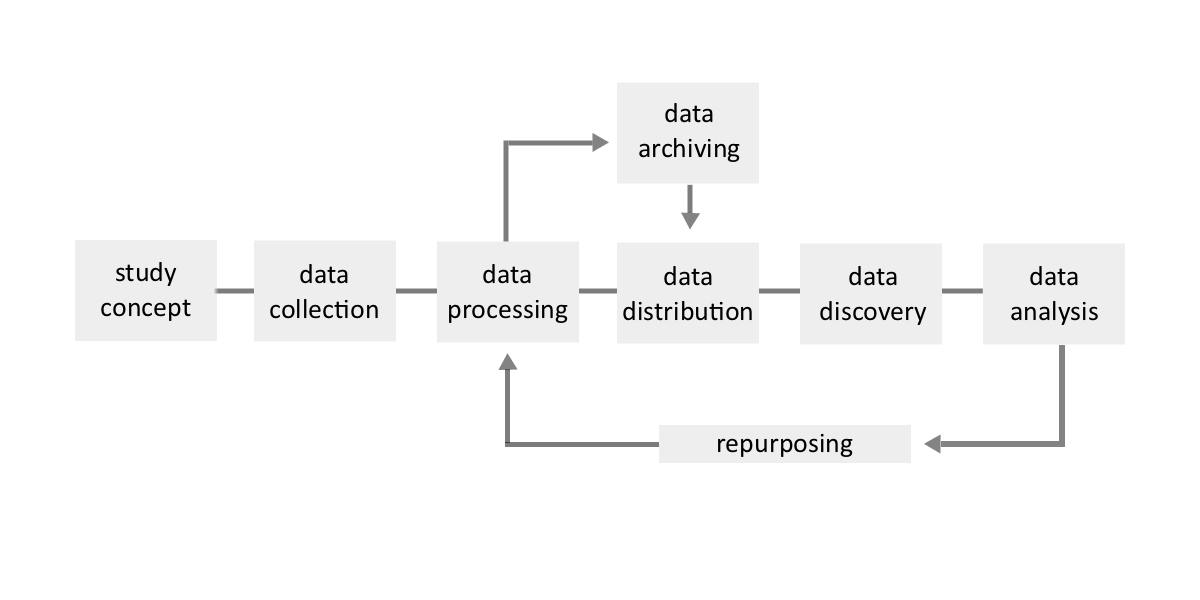
\includegraphics{https://raw.github.com/michellehudson/datamanagement/master/images/ddilifecycle.png}
\caption{DDI lifecycle model}
\end{figure}

\section{General format:}\label{general-format}

Using the DDI data lifecycle model as a guide, we'll cover the following
questions:

\begin{enumerate}
\def\labelenumi{\arabic{enumi}.}
\itemsep1pt\parskip0pt\parsep0pt
\item
  What does this stage of the data lifecycle involve?
\item
  What resources are available for doing it well at Yale (\& elsewhere)?
\item
  What are guidelines for managing data at this stage?
\end{enumerate}

\section{Outline:}\label{outline}

\begin{enumerate}
\def\labelenumi{\arabic{enumi}.}
\itemsep1pt\parskip0pt\parsep0pt
\item
  What is data?
\item
  Why manage it?
\item
  Study concept
\item
  Data collection
\item
  Data processing
\item
  Data archiving
\item
  Data distribution
\item
  More resources
\item
  Q\&A
\end{enumerate}

\section{What is research data?}\label{what-is-research-data}

Research data is defined as ``the recorded factual material commonly
accepted in the scientific community as necessary to validate research
findings.'' OMB Circular citation.

There are four types of research data:

\begin{enumerate}
\def\labelenumi{\arabic{enumi}.}
\itemsep1pt\parskip0pt\parsep0pt
\item
  Observational: captured in real time, usually irreplaceable (sensor
  readings, telescope images, sample data, surveys).
\item
  Experimental: data from lab equipment, can be reproducible but may be
  expensive (gene sequences).
\item
  Simulation: data generated from test models (climate models).
\item
  Derived or compiled: reproducible but expensive (data mining, compiled
  databases).
\end{enumerate}

Research data comes in many formats of information: documents,
spreadsheets, field notebooks, survey responses, audio and video
recordings, images, film, specimens, software code, and can be
structured and stored in a variety of file formats.

\section{Why manage research data?}\label{why-manage-research-data}

There are many reasons why good data management is important for your
research career, ranging from long-term effects on the future of science
to personal productivity and accomplishment.

\subsection{Transparency, integrity, and
reproducibility:}\label{transparency-integrity-and-reproducibility}

Managing data and making it accessible by peers decreases the chances of
an article being retracted because of falsified or missing data sets.
Reproducibility is a fundamental part of scientific research, and
failing to make all the components of a research study available makes
reproducibility impossible.

\subsection{Compliance:}\label{compliance}

Data management plans are required by funding agencies, and there is
increased expectation that the products of federal funding will be
required to be accessible to the public. In addition, many journals are
requiring data deposit before an article may be published.

\subsection{Personal \& professional
benefits:}\label{personal-professional-benefits}

If data is managed within your lab, research group, or simply
well-organized for your own use, you will save time, energy, and
resources. All members of the team will have an understanding of the
well-documented processing and analysis of the project's data, and be
able to carry out their research components more effectively. Sharing
research data is now regarded as an integral and valuable part of the
research process, and archiving your data in a repository will allow
other researchers to build upon your work and cite you in the process.

\section{Study concept}\label{study-concept}

\subsection{What does this stage
involve?}\label{what-does-this-stage-involve}

This is the pre-planning process for a study. It involves formulating a
research question and deciding on the methods you want to use to execute
your study. It may include submitting a grant to get funding. Some
grants require data management plans to be submitted as part of the
proposal.

\subsection{What tools and resources are
available?}\label{what-tools-and-resources-are-available}

\paragraph{\href{https://dmp.cdlib.org/}{DMPTool}:}\label{dmptool}

Yale is a DMPTool partner. Logging in with your Yale ID and password
will give you access to the DMPTool, which will give you an overview of
funder requirements (for various NSF, NIH, and other directorates and
divisions), and walk you through building a data management plan, asking
the right questions along the way. In the next iteration of the tool,
we'll be able to further customize it with Yale-specific resources.

\paragraph{\href{http://csssi.yale.edu/dmp}{DMP Consultation
Group}:}\label{dmp-consultation-group}

If you have to submit a DMP as part of a grant proposal and have trouble
using the DMPTool or answering questions you think are critical to the
good management of data, you can contact the DMP Consultation Group for
help. This group can review written plans and offer feedback, or connect
you with more resources at Yale you might be able to cite or consider
including in your plan to make a stronger proposal.

\paragraph{\href{http://csssi.yale.edu/csssi-statistical-consultants-schedule}{StatLab
consultants}:}\label{statlab-consultants}

Even if you aren't submitting a grant proposal, it's a good idea to come
to the StatLab at the beginning of your project. If you know what
analyses you want to do on your data, the StatLab can make sure you set
out to collect your data correctly. If you anticipate using StatLab
services near the end of your project, it's much easier for them if you
connect in the beginning of the project, as well.

\section{Data collection \&
documentation}\label{data-collection-documentation}

\subsection{What does this stage
involve?}\label{what-does-this-stage-involve-1}

This stage involves all the collection and subsequent documentation of
your data, and may involve collaboration with other people. There aren't
a lot of collaborative online spaces for data collection, but we can
discuss a few, and some general guidelines for documenting your research
well.

\subsection{Study-level description}\label{study-level-description}

\begin{enumerate}
\def\labelenumi{\arabic{enumi}.}
\itemsep1pt\parskip0pt\parsep0pt
\item
  Context of the data collection (project history, aim, objectives, and
  hypotheses)
\item
  Data collection methods (sampling, data collection process,
  instruments used, hardware and software used to collect data, scale
  and resolution, temporal and geographic coverage, secondary data
  sources used, if any)
\item
  Data set structure -- of files, study cases, and relationships between
  files
\item
  Changes made to data over time
\item
  Information on access and use conditions or data confidentiality
\end{enumerate}

\subsection{File-level description}\label{file-level-description}

\begin{enumerate}
\def\labelenumi{\arabic{enumi}.}
\itemsep1pt\parskip0pt\parsep0pt
\item
  Names, labels, and descriptions for variables, records, and their
  values
\item
  Definition of codes \& classification schemes used
\item
  Codes of and reasons for missing values
\end{enumerate}

\subsection{What tools and resources are
available?}\label{what-tools-and-resources-are-available-1}

Yale-supported:

\paragraph{\href{http://its.yale.edu/services/collaboration-and-file-sharing/box-yale}{Box}:}\label{box}

\paragraph{\href{http://its.yale.edu/services/research-technologies/elab-notebook/labarchives-faqs}{LabArchives}:}\label{labarchives}

\paragraph{\href{http://its.yale.edu/services/email-and-calendars/eliapps-google-apps-education}{EliApps}:}\label{eliapps}

\paragraph{\href{http://its.yale.edu/services/web-and-application-services/qualtrics-survey-tool}{Qualtrics}:}\label{qualtrics}

Additional services \& software:

\paragraph{\href{https://github.com/}{GitHub}:}\label{github}

\paragraph{\href{https://knb.ecoinformatics.org/morphoportal.jsp}{Morpho}:}\label{morpho}

\paragraph{\href{http://earthcube.org/}{Earthcube}:}\label{earthcube}

\paragraph{\href{http://www.colectica.com/}{Colectica}:}\label{colectica}

\subsection{Guidelines:}\label{guidelines}

\begin{itemize}
\itemsep1pt\parskip0pt\parsep0pt
\item
  Spreadsheets vs.~databases (plug workshop)
\item
  Consistency
\item
  Level of detail
\end{itemize}

\subsection{Example:}\label{example}

The codebook for the \href{http://www3.norc.org/GSS+Website/}{General
Social Survey} is \ldots{}

\section{Data processing \& analysis}\label{data-processing-analysis}

\subsection{What does this stage
involve?}\label{what-does-this-stage-involve-2}

These stages are in separate boxes on the lifecycle model, and they may
indeed be different steps, but not always. You usually process data in
order to get to an analyzable form of it. The stages have the same
considerations. This stage includes any data cleaning, refinement,
integration, and organizing (combining variables, weighting variables)
that you might do, as well as any computation necessary for analysis.

\subsection{What tools and resources are
available?}\label{what-tools-and-resources-are-available-2}

\paragraph{\href{http://csssi.yale.edu/tech}{Software}:}\label{software}

\begin{itemize}
\itemsep1pt\parskip0pt\parsep0pt
\item
  Stata
\item
  SAS
\item
  MatLab
\item
  R
\item
  OpenRefine
\item
  Python
\item
  \href{http://www.dataone.org/software_tools_catalog}{DataONE software
  tools catalog}
\end{itemize}

\paragraph{\href{http://its.yale.edu/services/research-technologies/high-performance-computing}{High
Performance Computing}:}\label{high-performance-computing}

\paragraph{\href{http://guides.library.yale.edu/gis}{Geographic
Information Systems}:}\label{geographic-information-systems}

\paragraph{Workflow tools}\label{workflow-tools}

\begin{itemize}
\itemsep1pt\parskip0pt\parsep0pt
\item
  \href{https://kepler-project.org/}{Kepler}:
\item
  \href{http://www.vistrails.org/index.php/Main_Page}{VisTrails}:
\end{itemize}

\subsection{People:}\label{people}

\paragraph{Steve Weston, HPC
specialist}\label{steve-weston-hpc-specialist}

Steve has office hours in the CSSSI from 9:30 - 1:00 on Wednesdays.
\#\#\#\# Stace Maples, GIS specialist Stace has office hours in the
CSSSI \#\#\#\# StatLab consultants: StatLab consultants staff a desk in
the CSSSI from 9:30 - 9:30. \#\#\#\# Kristin Bogdan \& Michelle Hudson,
Data Librarians Kristin \& Michelle have offices in CSSSI, and you can
see their offsite office hours at:

\subsection{Guidelines:}\label{guidelines-1}

\begin{enumerate}
\def\labelenumi{\arabic{enumi}.}
\itemsep1pt\parskip0pt\parsep0pt
\item
  Keep track of everything you do.
\item
  Best practices for working with data during analysis -- folder
  structures, naming conventions, statistical package considerations.
\item
  How to back up data
\end{enumerate}

\section{Data archiving \&
preservation}\label{data-archiving-preservation}

\subsection{What does this stage
involve?}\label{what-does-this-stage-involve-3}

Archiving and preserving research data is different from distributing it
or backing it up regularly. Preservation ensures long-term retention of
the data and the necessary migration from format to format that will be
required to keep the data usable over a time period. How long you retain
your data is often up to what your funding dictates -- some grants say
three years, others five. In some cases, your data may have value for an
indefinite period of time.

\subsection{What tools and resources are
available?}\label{what-tools-and-resources-are-available-3}

\paragraph{Lists of repositories}\label{lists-of-repositories}

1 2 3

\subsection{Guidelines:}\label{guidelines-2}

\begin{enumerate}
\def\labelenumi{\arabic{enumi}.}
\itemsep1pt\parskip0pt\parsep0pt
\item
  Best to hand it over completely, if complete, and let an institution
  take care of it for you.
\end{enumerate}

\subsection{Examples:}\label{examples}

ISPS data archive ICPSR

\section{Data distribution \&
citation}\label{data-distribution-citation}

\subsection{What does this stage
involve?}\label{what-does-this-stage-involve-4}

\subsection{What tools and resources are
available?}\label{what-tools-and-resources-are-available-4}

\paragraph{DataCite}\label{datacite}

\paragraph{EliScholar}\label{elischolar}

\paragraph{Other repositories}\label{other-repositories}

\subsection{Guidelines:}\label{guidelines-3}

\begin{enumerate}
\def\labelenumi{\arabic{enumi}.}
\itemsep1pt\parskip0pt\parsep0pt
\item
  Give your data set a title and make it easy to credit you.
\item
  Always cite data that you use as if it were as important as the
  journal articles you cite.
\end{enumerate}

\subsection{Examples:}\label{examples-1}

\begin{enumerate}
\def\labelenumi{\arabic{enumi}.}
\itemsep1pt\parskip0pt\parsep0pt
\item
  ICPSR data citation
\end{enumerate}

\section{References \& other
resources:}\label{references-other-resources}

\subsubsection{NEDMC}\label{nedmc}

\subsubsection{MANTRA}\label{mantra}

\subsubsection{Libguides}\label{libguides}

\section{Contact info}\label{contact-info}

\end{document}
